\documentclass[conference,10pt]{IEEEtran}
\IEEEoverridecommandlockouts
\usepackage{cite,amsmath,amssymb,graphicx,booktabs,url,algorithm,algpseudocode}
\usepackage[caption=false,font=footnotesize]{subfig}
\usepackage{float}
\usepackage{flafter}
\setcounter{dbltopnumber}{2}
\renewcommand{\dbltopfraction}{0.9}
\renewcommand{\dblfloatpagefraction}{0.8}
\usepackage[draft,hidelinks]{hyperref}

\title{Self-Organising Maps for Network Intrusion Categorisation}

\author{\IEEEauthorblockN{26946777}
\IEEEauthorblockA{RW 741 Machine Learning\\
Department of Computer Science, Stellenbosch University}}

\begin{document}
\maketitle

\begin{abstract}
Network intrusion detection requires a classifier that recognises rare attack categories as well as benign traffic.
The present study trains a self-organising map (SOM) on the UNSW-NB15 data set without the category label and attaches the label to the trained map.
The input representation, the lattice size, the training settings and the labelling rule are selected on a validation portion.
The selected map is compared with the nearest-neighbour classifier and the classification tree of Assignment 2 under stratified five-fold cross-validation.
The SOM requires a logarithmic transform and standardisation of the numeric inputs.
The validation macro F-measure shows a plateau from roughly 576 units, while the quantisation error continues to decrease.
Clustering of the codebook lowers the macro F-measure at every number of clusters.
An inverse-frequency vote detects most rows of the rarest category, although with a very low precision.
The SOM attains a macro F-measure of 0.4135, compared with 0.4525 for nearest neighbours and 0.5772 for the tree.
The class-weighted tree therefore remains the best model under the macro F-measure.
\end{abstract}

\let\thefootnote\relax
\footnotetext{The code that produced the results reported here is available at \url{https://github.com/naturalza/MLA-Assignment-4}.}

\begin{IEEEkeywords}
self-organising map, vector quantisation, network intrusion detection, class imbalance
\end{IEEEkeywords}

\section{Introduction}
A network intrusion detector assigns each traffic record to either benign traffic or one of nine families of attack.
In the UNSW-NB15 data set of Moustafa and Slay \cite{moustafa2015}, the benign category accounts for more than half of the records after duplicate removal.
The rarest attack family accounts for about one record in a thousand.
Consequently, a score that counts correct records rewards a detector that ignores the rare families \cite{he2009}.
The present study therefore uses the macro F-measure, defined as the unweighted mean of the per-category F-measures, as the primary score.

A self-organising map (SOM) offers an unsupervised route to the same task.
Kohonen placed the units of a SOM on a lattice and assigned each unit a codebook vector in the input space \cite{kohonen1990}.
Training moves the codebook vectors towards the data without reference to the category label.
Similar records therefore select neighbouring units, and the label is attached to the units only after training.
A new record receives the category attached to the closest unit.
Kayacik \emph{et al.} and Ramadas \emph{et al.} showed that SOMs separate normal and anomalous network traffic without supervision \cite{kayacik2007,ramadas2003}.

The study compares a tuned SOM with the two classifiers of Assignment 2, namely a nearest-neighbour classifier and a classification tree.
Four research questions direct the study.
The first question asks for the smallest lattice on the plateau of the validation macro F-measure.
The second question asks whether clustering of the codebook vectors yields better category labels than the majority category of each unit.
The third question asks whether a class cap during training or a weighted vote after training reduces the dominance of the largest category.
The fourth question asks how the selected SOM compares with the two classifiers of Assignment 2 on identical cross-validation folds.

The main conclusion of the study is that the SOM does not match the class-weighted tree under the macro F-measure.
The SOM requires a logarithm and standardisation of the numeric inputs, and the validation score shows a plateau from roughly 576 units.
Clustering of the codebook lowers the score, because each of the three largest categories occupies more than one region of the map.
An inverse-frequency vote detects most rows of the rarest category, but the precision of the vote on that category is very low.

The remainder of the report is organised as follows.
Section~\ref{sec:background} presents the SOM and the rules that attach labels to the SOM.
The same section presents the reference classifiers, the performance measures and the data set.
Section~\ref{sec:implementation} describes the implementation.
Section~\ref{sec:empirical} sets out the empirical process and the selection rules.
Section~\ref{sec:results} reports and discusses the results.
Section~\ref{sec:conclusions} concludes the report.

\section{Background}
\label{sec:background}
The purpose of the present section is to define every model and measure used in the study.
The section first defines vector quantisation and the SOM.
The section also defines the labelling of the codebook vectors, the reference classifiers, and the performance measures.
The section closes with the properties of the data set and the expectations that follow from those properties.

\subsection{Vector quantisation}
Engelbrecht described a vector quantiser as the replacement of many patterns by a smaller set of codebook vectors \cite{engelbrecht2007}.
Let $\mathbf{z}_p$ denote the input vector of training pattern $p$, and let $P$ denote the number of training patterns.
Each unit $u$ holds a codebook vector $\mathbf{w}_u$.
The best-matching unit $b(p)$ of pattern $p$ is the unit with the smallest squared Euclidean distance $\lVert\mathbf{z}_p-\mathbf{w}_u\rVert_2^2$.
The quantisation error over the training patterns is
\begin{equation}
Q=\frac{1}{P}\sum_{p=1}^{P}\lVert\mathbf{z}_p-\mathbf{w}_{b(p)}\rVert_2^2.
\label{eq:qe}
\end{equation}
A small value of $Q$ indicates that the codebook vectors lie close to the patterns.
However, a small value of $Q$ does not guarantee a correct category label, because $Q$ ignores the label entirely.

\subsection{Self-organising map}
The SOM is a vector quantiser with the units arranged on a lattice \cite{kohonen1990,kohonen2001}.
The present study uses a rectangular lattice, and $\mathbf{g}_u$ denotes the lattice coordinate of unit $u$.
Kohonen also used a hexagonal lattice \cite{kohonen1990}.
The rectangle was preferred because the growth rule of Engelbrecht inserts whole rows and columns \cite{engelbrecht2007}.

During training, the units compete for each pattern, and the best-matching unit $v=b(p)$ wins.
The neighbourhood kernel between the winner $v$ and unit $u$ at epoch $t$ is
\begin{equation}
\phi_{vu}(t)=\exp\left(-\frac{\lVert\mathbf{g}_v-\mathbf{g}_u\rVert_2^2}{2\sigma^2(t)}\right),
\label{eq:kernel}
\end{equation}
where $\sigma(t)$ is the neighbourhood width.
Kohonen moved the winner and the neighbours of the winner towards the pattern \cite{kohonen1990}, so that
\begin{equation}
\mathbf{w}_u\leftarrow\mathbf{w}_u+\eta(t)\,\phi_{vu}(t)\left(\mathbf{z}_p-\mathbf{w}_u\right),
\label{eq:update}
\end{equation}
where $\eta(t)$ is the learning rate.
The width and the learning rate decay as
\begin{equation}
\sigma(t)=\sigma(0)\,e^{-t/\tau},\qquad\eta(t)=\eta(0)\,e^{-t/\tau},
\label{eq:decay}
\end{equation}
with a time constant $\tau$ shared by both decays.
Repeated presentation moves codebook vectors into dense regions of the input space.
As a result, a region with few patterns receives few codebook vectors \cite{kohonen2001}.

Engelbrecht separated training into an ordering phase and a convergence phase \cite{engelbrecht2007}.
The ordering phase starts with a width that spans the lattice and a high learning rate, so that the lattice spreads over the data.
The convergence phase uses a narrow width and fine-tunes the codebook vectors.
Kohonen proposed the batch map for convergence \cite{kohonen2001}.
Let $n_v$ denote the number of training patterns won by unit $v$, and let $\bar{\mathbf{z}}_v$ denote the mean of those patterns.
The batch map replaces every codebook vector by the kernel-weighted mean
\begin{equation}
\mathbf{w}_u=\frac{\sum_{v}n_v\,\phi_{vu}(t)\,\bar{\mathbf{z}}_v}{\sum_{v}n_v\,\phi_{vu}(t)}.
\label{eq:batch}
\end{equation}
The batch map needs no learning rate.

Two measures describe a trained map.
The quantisation error in \eqref{eq:qe} measures the fit to the data.
Kiviluoto defined the topographic error as the fraction of patterns whose best and second-best units are not adjacent on the lattice \cite{kiviluoto1996}.
Let $b'(p)$ denote the second-best unit of pattern $p$, and let $\delta_p$ equal one when $b(p)$ and $b'(p)$ are not orthogonal neighbours and zero otherwise.
The topographic error is
\begin{equation}
T=\frac{1}{P}\sum_{p=1}^{P}\delta_p.
\label{eq:te}
\end{equation}
A low value of $T$ indicates that the lattice preserves the neighbourhood structure of the data.
Ultsch and Siemon displayed the distance between the codebook vectors of adjacent units as a unified distance matrix \cite{ultsch1990}.
Large distances in the unified distance matrix mark boundaries between groups of units.

Engelbrecht noted that a lattice with too few units forces unrelated patterns onto the same unit \cite{engelbrecht2007}.
Conversely, a lattice with as many units as patterns assigns a separate unit to each pattern and stops summarising the data.
The useful lattice size is therefore the smallest size where further units stop improving the category score.
The value of $Q$ always decreases as units are added, so $Q$ cannot identify that size.
When the score still improves at the largest lattice of a sweep, Engelbrecht grew the map instead \cite{engelbrecht2007}.
The growing map inserts a row and a column next to the unit with the largest quantisation error.
The insertion lies between that unit and the adjacent unit with the most distant codebook vector.
Each inserted codebook vector is the mean of the two codebook vectors on either side.

\subsection{Labelling of the codebook}
After training, each unit holds a histogram of the training categories of the patterns that the unit won.
The study compares three rules that convert the histograms into predictions.
The first rule assigns each unit the majority category of the unit.
The second rule clusters the codebook vectors and assigns every unit in a cluster the majority category of the cluster.
The third rule combines the histograms of neighbouring units in a weighted vote at prediction time.

The second rule uses the hierarchical criterion of Ward \cite{ward1963}.
At each step, Ward merged the two clusters whose union produces the smallest increase in the within-cluster sum of squared errors.
For clusters $A$ and $B$, the increase is
\begin{equation}
d_{AB}=\frac{n_A n_B}{n_A+n_B}\lVert\boldsymbol{\mu}_A-\boldsymbol{\mu}_B\rVert_2^2,
\label{eq:ward}
\end{equation}
where $n_A$ is the number of training patterns won by the units in cluster $A$, and $\boldsymbol{\mu}_A$ is the pattern-weighted mean of the codebook vectors in $A$.
Initially, each occupied unit forms a cluster of one unit.
Vesanto and Alhoniemi merged only clusters that share a lattice edge \cite{vesanto2000}.
The constraint keeps every cluster a connected region of the map.
The number of clusters is a control parameter of the second rule.
A number equal to the number of categories assumes that each category occupies a single region, and the validation score tests that assumption.

The third rule is an inverse-frequency vote.
Let $C$ denote the number of categories, and let $m_c$ denote the number of training patterns in category $c$.
The weight of category $c$ is
\begin{equation}
\alpha_c=\frac{P}{C\,m_c}.
\label{eq:weight}
\end{equation}
A query first finds the best-matching unit $v$.
The vote for category $c$ is the sum of the histogram counts of $c$ over every unit $u$ within three widths of $v$.
Each count is multiplied by $\phi_{vu}$ and by $\alpha_c$.
The weight raises the influence of a rare category, as He and Garcia recommended for imbalanced data \cite{he2009}.

Two conventions keep every prediction defined.
A tie in a vote goes to the category with the larger training count.
A unit that won no training pattern takes the category of the nearest named unit on the lattice.

\subsection{Reference classifiers}
The reference classifiers are the two models of Assignment 2.
Both models are restated here, so that the comparison does not depend on the earlier report.

Cover and Hart assigned a new pattern the majority category among the $k$ nearest training patterns under Euclidean distance \cite{cover1967}.
Hastie \emph{et al.} noted that the contribution of an input to the Euclidean distance grows with the range of the input \cite{hastie2009}.
Inputs with wide ranges therefore dominate the vote unless the inputs are rescaled.
In Assignment 2, a grid search under stratified five-fold cross-validation compared values of $k$ from one to 50 with uniform and distance-weighted votes.
The macro F-measure selected $k=7$ with a uniform vote, and distance weighting gave no improvement at any value of $k$.
The same authors noted that a small value of $k$ follows the local structure of the data but responds strongly to noise \cite{hastie2009}.
A large value of $k$ smooths the decision boundary, but the frequent categories dominate a large neighbourhood.
The uniform vote gives each of the seven neighbours one vote.
The present study adds a weighted vote that gives a neighbour of category $c$ the weight $\alpha_c$ from \eqref{eq:weight}.
Both votes use the same seven neighbours, so the weight is the only difference.

Breiman \emph{et al.} partitioned the input space by a threshold on one input at a time \cite{breiman1984}.
Let $\theta_c$ denote the weighted share of category $c$ among the training patterns at a node.
The Gini index of the node is
\begin{equation}
G=1-\sum_{c=1}^{C}\theta_c^2.
\label{eq:gini}
\end{equation}
The tree selects the threshold that maximises the decrease $G-(\omega_L G_L+\omega_R G_R)/\omega$.
Here, $\omega$ is the total pattern weight at the node.
The symbols $\omega_L$ and $G_L$ denote the weight and the Gini index of the left child, and $\omega_R$ and $G_R$ denote those of the right child.
A threshold on one input is unaffected by a monotone rescaling of that input, so the tree needs neither a logarithm nor standardisation.
Breiman \emph{et al.} controlled the size of a tree to prevent the tree from fitting individual training patterns \cite{breiman1984}.
In the present study, the maximum depth serves that purpose.
The minimum leaf size sets how few patterns a leaf may describe, and a small minimum allows a leaf that isolates a rare category.
Class weighting raises the contribution of the rare categories to the Gini index.
In Assignment 2, the grid compared the Gini index and entropy at depths from five to 25 and without a limit, followed by leaf sizes and class weighting.
The macro F-measure selected the Gini index, a maximum depth of 15, a minimum of one pattern per leaf, and class weighting.
Each training pattern of category $c$ carries the weight $\alpha_c$.

\subsection{Performance measures}
Sokolova and Lapalme showed that accuracy favours the majority category when the categories are imbalanced \cite{sokolova2009}.
The study therefore reports three measures.
The precision $\pi_c$ of category $c$ is the fraction of patterns predicted as $c$ that belong to $c$.
The recall $\rho_c$ is the fraction of patterns of category $c$ that are predicted as $c$.
The F-measure of category $c$ is
\begin{equation}
F_c=\frac{2\pi_c\rho_c}{\pi_c+\rho_c},
\label{eq:f}
\end{equation}
and $F_c$ is zero when $\pi_c+\rho_c$ is zero.
The macro F-measure is
\begin{equation}
\bar{F}=\frac{1}{C}\sum_{c=1}^{C}F_c.
\label{eq:macro}
\end{equation}
Every category contributes equally to $\bar{F}$, regardless of size.
Brodersen \emph{et al.} defined the balanced accuracy $\bar{\rho}$ as the unweighted mean of the per-category recalls \cite{brodersen2010}.
Accuracy, the fraction of correctly classified patterns, is the third measure.

\subsection{Properties of the data set}
Moustafa and Slay released the UNSW-NB15 data set \cite{moustafa2015,moustafa2016}.
Each record carries an identifier, 42 inputs, a binary attack flag and a category label.
Three of the inputs are nominal and 39 are numeric.
In decreasing order of size, the 10 categories are Normal, Exploits, Fuzzers, Reconnaissance, Generic, denial of service (DoS), Analysis, Backdoor, Shellcode and Worms.
The identifier is unique to each row.
A distance that includes the identifier therefore separates every training row and matches no new row.
The binary flag is a coarser copy of the category label and would leak the target into the inputs.
Both columns are removed before any other step.
Exact duplicate rows remain after the identifier is removed.
A duplicate places the same observation in both a training partition and an evaluation partition, and the score rewards memorisation.
For the SOM and the nearest-neighbour vote, the evaluation copy lies at distance zero from the training copy.
For the tree, the evaluation copy reaches the leaf fitted to the training copy.
Duplicates are therefore removed before any split.

The ranges of the numeric inputs span nine orders of magnitude, as Assignment 2 reported.
Under Euclidean distance, the widest input decides the best-matching unit.
Standardisation subtracts the training mean of each numeric input and divides the result by the training standard deviation of that input.
Standardisation equalises the scales of the inputs and does not assume a normal distribution.
However, extreme values of a right-skewed input dominate the standard deviation of that input.
In Assignment 2, 14 of the 39 numeric inputs had more than five per cent of the values beyond three interquartile ranges from the quartiles.
The natural logarithm of one plus the value compresses a right-skewed, non-negative input and maps a zero value to zero.
The logarithm is therefore applied before standardisation.
A logarithm changes the mean that a codebook vector stores.
The study therefore tests whether the logarithm is necessary for the SOM.

Normal traffic accounts for 85\,722 of the 162\,745 deduplicated rows, a share of 52.67 per cent.
Worms is the smallest category, with 171 rows.
A SOM that follows the density of the data assigns most units to the largest category.
As a result, a rare category shares units with frequent categories and loses the majority vote on those units.
The SOM is therefore expected to show a reasonable accuracy and a weak macro F-measure.
The macro F-measure of the SOM is expected to lie near that of the uniform nearest-neighbour vote and below that of the weighted tree.
Two remedies leave the training of the SOM unsupervised.
The first remedy is the inverse-frequency vote.
The second remedy caps the number of training patterns per category during training.

The imbalance affects the reference classifiers in the same way.
A neighbourhood drawn from a region dominated by a frequent category rarely contains enough rare patterns to win the uniform vote.
The weighted vote is the remedy for the nearest-neighbour classifier.
In an unweighted tree, the frequent categories dominate the Gini index, so a split that isolates a rare category yields little decrease in $G$.
The class weight $\alpha_c$ is the remedy for the tree.

Finally, identical input vectors occur with different category labels in the data set.
No classifier restricted to the inputs can separate the rows that share such a vector.
Assignment of the majority category of each distinct vector to every copy gives an upper bound on accuracy.

In summary, the SOM is a density-following vector quantiser, and labels enter only after training.
The class imbalance of the data set leads to the expectation that the SOM will favour the frequent categories.

\section{Implementation}
\label{sec:implementation}
The present section describes how the models were implemented.
The section presents the training procedure of the SOM, the labelling procedure, and the reference classifiers.
All models were written in Python with the NumPy library \cite{harris2020} and the Numba compiler \cite{lam2015}.
No machine learning library supplied any reported model.

\subsection{Training procedure}
Algorithm~\ref{alg:train} lists the two-phase training procedure.
The initial codebook vectors are drawn from distinct training patterns, so every unit starts inside the region occupied by the data.
The initial width $\sigma(0)$ is half the longer side of the lattice, so the first neighbourhood spans the lattice.
The ordering phase lasts $E=8$ epochs.
The time constant is $\tau=E/\ln\sigma(0)$, so the width decays to one at the first convergence epoch.
The initial learning rate is $\eta(0)=0.5$.
By default, the convergence phase holds the width at one.
A width of zero would reduce the weighted vote to the majority rule, so the width is kept above zero.
Units more than three widths from the winner are not updated, because the kernel in \eqref{eq:kernel} is below 0.012 at that distance.
The convergence phase stops when the relative decrease in $Q$ stays below $10^{-4}$ for five consecutive epochs, or after 25 epochs.

\begin{algorithm}[tb]
\caption{Two-phase training of the map}
\label{alg:train}
\begin{algorithmic}[1]
\State Set each codebook vector to a distinct, randomly drawn training pattern
\For{each ordering epoch $t$ from zero to $E-1$}
  \State Compute $\sigma(t)$ and $\eta(t)$ by \eqref{eq:decay}
  \For{each training pattern, in a new random order}
    \State Find the best-matching unit
    \State Update every unit within three widths by \eqref{eq:update}
  \EndFor
\EndFor
\Repeat
  \State Assign every training pattern to the best-matching unit
  \State Compute the count and the mean of the patterns of each unit
  \State Replace every codebook vector by \eqref{eq:batch} at the convergence width
\Until{the stopping rule holds}
\end{algorithmic}
\end{algorithm}

A growing map starts from the largest lattice of the sweep.
Each insertion adds a row and a column next to the unit with the largest quantisation error.
After each insertion, three ordering epochs and the convergence phase retrain the map.

\subsection{Labelling procedure}
The histograms count the training patterns of each category won by each unit.
Algorithm~\ref{alg:vote} lists the inverse-frequency vote.
The majority rule and the cluster rule use the same histograms.
The cluster rule merges occupied units under \eqref{eq:ward} and the lattice-edge constraint until the required number of clusters remains.

\begin{algorithm}[tb]
\caption{Inverse-frequency neighbourhood vote}
\label{alg:vote}
\begin{algorithmic}[1]
\State Find the best-matching unit $v$ of the query
\State Collect every unit $u$ within three widths of $v$
\For{each category $c$}
  \State Sum the count of $c$ at each collected unit $u$, multiplied by $\phi_{vu}$ and by $\alpha_c$
\EndFor
\State Predict the category with the largest sum
\State Break a tie in favour of the category with the larger training count
\end{algorithmic}
\end{algorithm}

\subsection{Reference classifiers}
The nearest-neighbour search computes squared Euclidean distances in blocks and keeps the seven nearest training patterns.
The uniform and the weighted votes read the same list of neighbours.
At each node, the tree scans every threshold of every input and keeps the threshold with the largest weighted decrease in $G$.
Unit tests on separable toy problems verified every model and both votes before the data set was used.
As a further check, the scores of both reference classifiers were compared with the scores reported in Assignment 2.

In summary, every model was implemented from first principles, and both reference classifiers were compared with the results of Assignment 2.

\section{Empirical process}
\label{sec:empirical}
The present section describes how the data were prepared and how the control parameters of the SOM were selected.
The section also describes the design of the final comparison.
Every selection rule was fixed before the corresponding score was observed.
Control parameters were selected on a single stratified split and remained fixed afterwards.
Kohavi recommended stratified cross-validation for estimates of generalisation \cite{kohavi1995}, so the frozen models were compared under stratified five-fold cross-validation.

\subsection{Data preparation}
The official training file of 175\,341 rows and the official testing file of 82\,332 rows were combined into a single table of 257\,673 rows.
The identifier and the binary attack flag were removed.
Exact duplicate rows were removed after the removal of the identifier, because a unique identifier makes every row distinct.
The table fell to 162\,745 rows, a reduction of 36.84 per cent.
Nominal levels seen fewer than 50 times in a training partition were collapsed into a single level.
A level with fewer than 50 rows forms less than 0.05 per cent of the training portion, so the level has almost no influence on a codebook vector or on a tree split.
In Assignment 2, 118 of the 133 levels of the protocol input occurred fewer than 50 times, and the same threshold keeps the two studies comparable.
The service value ``-'' denotes that no application protocol was recorded, and the value was kept as a separate level.
The nominal inputs were one-hot encoded, giving 72 inputs in total.
A nominal input has no order, so an integer code would impose an arbitrary distance between levels.
One-hot encoding places every pair of distinct levels at the same distance, as the Euclidean distance of the SOM and of the nearest-neighbour vote requires.
The tree tests numeric thresholds, and the one-hot encoding allows one threshold to isolate one level.

\subsection{Partitions}
The tuning split was stratified by category and shuffled with the seed 20261019.
The training portion held 70 per cent of the rows.
The validation portion and a held-out portion each held 15 per cent.
Training of the SOM and construction of the histograms used only the training portion.
Every selection used the validation portion.
The held-out portion was never scored, so that no second opportunity to select a model arose.

The generalisation comparison used a stratified five-fold partition of the full deduplicated table with the same seed.
The folds overlapped the tuning split, so the selection saw rows that later appeared in the test folds.
The overlap is a limitation of the design.
However, no control parameter changed after selection, and every model was retrained from scratch on each fold.

\subsection{Selection stages}
The stages ran in a fixed order, and each stage kept the choices of the earlier stages fixed.

\emph{Input representation:}
Three representations were compared on a lattice of $16\times16$ units with majority labels.
The first representation used the raw numeric inputs with the one-hot encoding.
The second representation standardised the numeric inputs.
The third representation applied the natural logarithm of one plus the value to every non-negative numeric input with an absolute skewness above two.
Standardisation followed the logarithm.
The threshold of two matches the threshold of Assignment 2, where 32 of the 39 numeric inputs exceeded the threshold.
The representation with the highest validation macro F-measure was selected.
On each generalisation fold, the skewed inputs and the standardisation statistics were recomputed from the training rows of that fold.
The tree always received the raw encoding, and the nearest-neighbour classifier always received the logarithm with standardisation, as in Assignment 2.

\emph{Lattice size:}
Square lattices with sides from eight to 40 units, in steps of four, were trained with the seed 20261019 and scored with majority labels.
The number of units therefore grew from 64 to 1\,600.
The largest lattice holds one unit for roughly every 70 training patterns, so every lattice still summarises the data.
The smallest lattice within 0.01 of the best validation macro F-measure was selected.
The band favours the smaller and faster lattice when a larger lattice improves the score by less than 0.01.
The values of $Q$ and $T$ were recorded but did not enter the selection.
Two further seeds, 20261020 and 20261021, were trained at the selected size.
The range of the three scores served as the initialisation noise in later stages.
Growth was triggered only when the selected size was the largest size in the sweep and the last step of the sweep improved the score by more than the noise.

\emph{Training settings:}
The settings $\eta(0)$, $E$ and the convergence width were varied one at a time at the selected size.
The number of ordering epochs and the convergence width were halved and doubled, giving four and 16 epochs and widths of 0.5 and two.
The learning rate took the values 0.1 and 0.9, on either side of the default and below the limit of one that \eqref{eq:update} requires.
An alternative replaced the default only when the alternative exceeded the default by more than the initialisation noise.

\emph{Labelling rule:}
The three labelling rules were scored on the selected map.
The cluster rule was evaluated at the cluster counts in the set $\{4,6,8,10,12,16,20,30,50,100,200\}$.
The counts ranged from four, below the number of categories, to 200, close to the number of occupied units.
The counts were densest near 10, where a structure of one region per category would appear.
The rule with the highest validation macro F-measure was selected.
A tie in the macro F-measure was broken by balanced accuracy.
A remaining tie favoured the simpler rule, and a tie between cluster counts favoured fewer clusters.

\emph{Class cap:}
A further SOM was trained when the validation recall of Worms under the best unweighted rule was below 0.2.
A recall of 0.2 corresponded to five of the 26 Worms rows in the validation portion.
A lower recall therefore indicated that the map ignored Worms.
The training of that SOM used at most 2\,000 training patterns from each category.
The cap limited the six categories with more than 2\,000 training patterns.
The four smallest categories kept every training pattern.
The histograms still used every training row.
The cap was adopted only when the cap raised the validation macro F-measure.

\subsection{Generalisation comparison}
The selected SOM, the tree, and both nearest-neighbour votes were retrained on the training rows of each of the five folds.
The SOM of each fold was initialised with the seed 20261019 plus the fold index, a number from zero to four.
The reported score of each model is the mean over the five folds, together with the population standard deviation of the five fold scores.
Per-category results pool the predictions of the five folds, so that each row is counted exactly once.

In summary, the selection proceeded in fixed stages on the validation portion, and the final comparison used five folds shared by all models.

\section{Results and discussion}
\label{sec:results}
The present section reports the outcome of each selection stage, followed by the generalisation comparison.
The stages appear in the order of execution.
The first subsections address the input representation, the lattice size, and the training settings.
The next subsections address the labelling rule and the class cap.
The generalisation comparison and the limit imposed by label ambiguity close the section.

\subsection{Input representation}
On a lattice of $16\times16$ units with majority labels, the raw encoding attained a validation macro F-measure of 0.1688.
Standardisation raised the score to 0.2821, and the logarithm followed by standardisation raised the score further to 0.3284.
The logarithm was therefore selected.
The quantisation error fell from $2.14\times10^{16}$ under the raw encoding to 6.14 under the selected representation.
The raw value of $Q$ showed that the inputs with the widest ranges determined every best-matching unit, as the Euclidean argument in the background predicted.
The gain from the logarithm showed that standardisation without the logarithm left the skewed inputs dominated by extreme values.
The same ordering of the three representations appeared for the nearest-neighbour classifier in Assignment 2.

\subsection{Lattice size}
Fig.~\ref{fig:size} reports the lattice sweep.
The quantisation error fell steadily from 11.58 at 64 units to 2.84 at 1\,600 units.
The topographic error stayed between 0.07 and 0.12 at every size, so the larger lattices preserved the neighbourhood structure as well as the smaller lattices.
The macro F-measure rose from 0.2563 at 64 units to 0.3842 at 576 units.
Beyond 576 units, the score fluctuated between 0.3760 and 0.3954 without a consistent trend.

\begin{figure*}[tb]
\centering
\subfloat[Quantisation error]{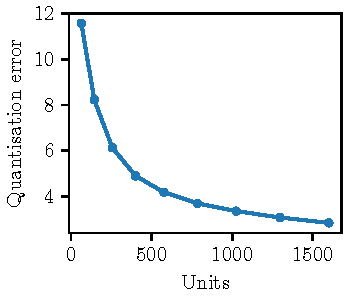
\includegraphics{figures/size_qe.pdf}}\hfill
\subfloat[Topographic error]{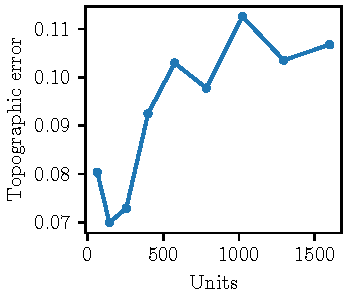
\includegraphics{figures/size_te.pdf}}\hfill
\subfloat[Validation macro F-measure]{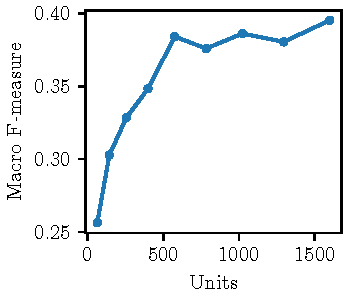
\includegraphics{figures/size_f.pdf}}
\caption{Measures of the trained map for each number of units}
\label{fig:size}
\end{figure*}

The best score of 0.3954 occurred at 1\,600 units.
The selection band therefore admitted every lattice with a score of at least 0.3854.
The smallest such lattice had 1\,024 units, and the $32\times32$ lattice was selected.
Three seeds at the selected size scored 0.3863, 0.3825 and 0.3752, a range of 0.0111.
The fluctuation beyond 576 units spanned 0.0194, less than twice the initialisation noise.
The sweep therefore showed a plateau from roughly 576 units, and the answer to the first research question is a lattice of between 576 and 1\,024 units.
Beyond the plateau, additional units continued to reduce $Q$ without improving the category score.
The selected size was not the largest size of the sweep, so the growth rule was not triggered.

\subsection{Training settings}
Table~\ref{tab:sense} reports the one-at-a-time variation of the training settings on the $32\times32$ lattice.
Both alternative learning rates and both alternative numbers of ordering epochs scored below the default.
The largest of those decreases was 0.0199, at a learning rate of 0.1.
The defaults for $\eta(0)$ and $E$ were therefore retained.

\begin{table}[tb]
\caption{Variation of the training settings on the selected lattice}
\label{tab:sense}
\centering
\footnotesize
\begin{tabular}{lcccc}
\toprule
Setting & Value & $Q$ & $T$ & $\bar{F}$ \\
\midrule
Default & --- & 3.36 & 0.113 & 0.3863 \\
$\eta(0)$ & 0.1 & 3.39 & 0.108 & 0.3664 \\
$\eta(0)$ & 0.9 & 3.36 & 0.108 & 0.3814 \\
$E$ & 4 & 3.38 & 0.114 & 0.3706 \\
$E$ & 16 & 3.38 & 0.109 & 0.3695 \\
Convergence width & 0.5 & 2.30 & 0.309 & 0.4072 \\
Convergence width & 2 & 5.75 & 0.067 & 0.3684 \\
\bottomrule
\end{tabular}
\end{table}

The convergence width had a much larger effect than the other two settings.
A width of 0.5 raised the validation macro F-measure by 0.0209, nearly twice the initialisation noise, and the width of 0.5 was adopted.
The narrow width also lowered $Q$ from 3.36 to 2.30 but nearly tripled $T$, from 0.113 to 0.309.
Conversely, a width of two lowered $T$ to 0.067 and lowered the score to 0.3684.
A narrow kernel lets each codebook vector move towards the patterns of a single unit, so the map fits the data more closely while the lattice becomes less ordered.
The category score therefore rewarded local fidelity over topology preservation.

\subsection{Labelling rule}
Table~\ref{tab:names} reports the validation scores of the three labelling rules on the selected map.
The inverse-frequency vote attained the highest macro F-measure of 0.4153, compared with 0.4072 for the majority rule.
The vote was therefore selected.
The gap of 0.0081 lay inside the initialisation noise.
However, the vote raised the balanced accuracy from 0.3886 to 0.5679 and the recall of Worms from zero to 0.692.
The secondary measures therefore favoured the same choice.
The validation portion contained 26 rows of Worms, and a recall of 0.692 corresponded to 18 of those rows.

\begin{table}[tb]
\caption{Validation scores of the labelling rules on the selected map}
\label{tab:names}
\centering
\footnotesize\setlength{\tabcolsep}{4pt}
\begin{tabular}{lcccc}
\toprule
Rule & $\bar{F}$ & $\bar{\rho}$ & Accuracy & Worms recall \\
\midrule
Majority & 0.4072 & 0.3886 & 0.7384 & 0 \\
Weighted vote & 0.4153 & 0.5679 & 0.6319 & 0.692 \\
Ward, 10 clusters & 0.2066 & 0.2000 & 0.5690 & 0 \\
Ward, 30 clusters & 0.2397 & 0.2609 & 0.6593 & 0 \\
Ward, 100 clusters & 0.3128 & 0.3139 & 0.7108 & 0 \\
Ward, 200 clusters & 0.3485 & 0.3383 & 0.7186 & 0 \\
\bottomrule
\end{tabular}
\end{table}

Every clustering scored below both unit-level rules.
The score of the cluster rule rose almost monotonically, from 0.0690 at four clusters to 0.3485 at 200 clusters.
The cut at 10 clusters, one cluster per category, scored only 0.2066.
When every occupied unit forms a cluster of one unit, the cluster rule coincides with the majority rule, with a score of 0.4072.
The steady rise showed that every merge discarded category information, and no number of clusters below the number of occupied units was optimal.
The answer to the second research question is therefore negative.
Clustering of the codebook did not improve on the majority category of each unit.

Fig.~\ref{fig:map} explains the negative result.
The majority categories in Fig.~\ref{fig:map}(a) form one compact region for Generic, but Normal, Exploits and Fuzzers each occupy more than one region.
The unified distance matrix in Fig.~\ref{fig:map}(b) shows narrow ridges of large distance.
Only 13.9 per cent of the units had a mean neighbour distance above twice the median, and the remainder of the map showed small and uniform distances.
A merge that respects the distances therefore joins neighbouring units of different categories.
As a result, the minority category of the merged region loses the label.
The categories of the data set thus did not form single connected regions of the input space, contrary to the assumption behind a cut at 10 clusters.

\begin{figure*}[tb]
\centering
\subfloat[Majority category of each unit]{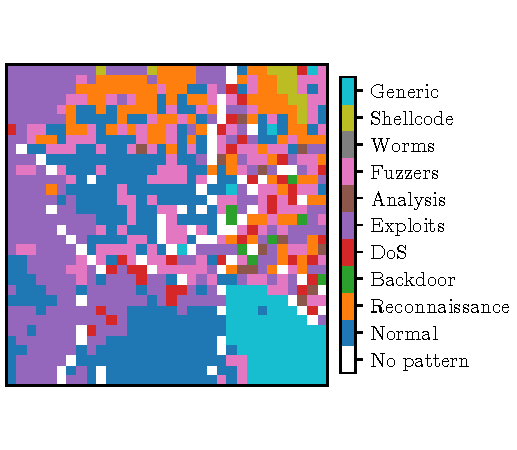
\includegraphics{figures/map.pdf}}\hfill
\subfloat[Unified distance matrix]{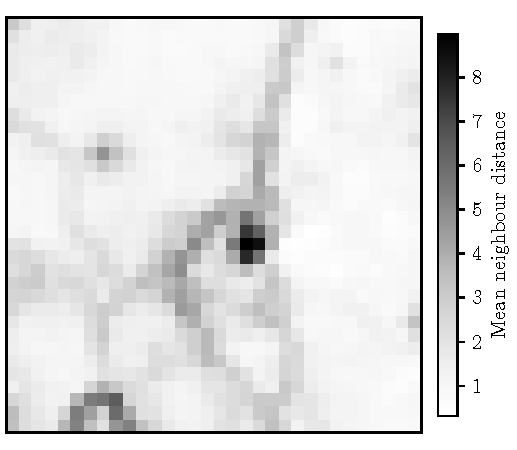
\includegraphics{figures/umatrix.pdf}}
\caption{Structure of the selected map}
\label{fig:map}
\end{figure*}

\subsection{Class cap}
The majority rule left the recall of Worms at zero, below the threshold of 0.2, so the capped map was trained.
The capped map attained a validation macro F-measure of 0.4170 under the inverse-frequency vote, compared with 0.4153 without the cap.
Under the rule declared in advance, the cap was adopted.
However, the gain of 0.0017 was about one sixth of the initialisation noise, so the evidence did not show that the cap improved the macro F-measure.
The cap did raise the validation recall of Worms from 0.692 to 0.808.

The cap changed the allocation of units more than the score.
Of the 1\,024 units of the selected map, 70 won no training pattern.
Normal held the majority on 271 units, or 26.5 per cent of the units, although Normal accounts for 52.67 per cent of the rows.
Exploits held the majority on 274 units and Fuzzers on 153 units.
Backdoor, Analysis and Shellcode held the majority on eight, 12 and 13 units respectively.
Worms held the majority on no unit, and the 120 training rows of Worms fell on 63 different units.
Every correct Worms prediction therefore came from the weighted vote rather than from a unit label.

Fig.~\ref{fig:qe} shows the training trace of the selected map.
The ordering phase reduced $Q$ on the capped draw from 22.83 to 3.83.
The convergence phase reduced $Q$ further to 1.87 and met the tolerance rule after 19 epochs.
The answer to the third research question is that both remedies changed the behaviour of the map on the rare categories.
However, only the inverse-frequency vote produced correct predictions of Worms, and neither remedy produced a gain in macro F-measure larger than the noise.

\begin{figure}[tb]
\centering
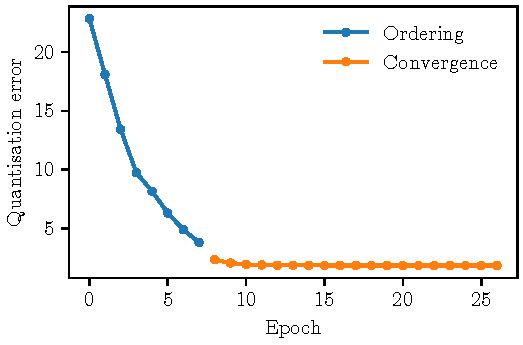
\includegraphics{figures/qe.pdf}
\caption{Quantisation error of the selected map during training}
\label{fig:qe}
\end{figure}

\subsection{Generalisation comparison}
Table~\ref{tab:final} reports the five-fold scores of the selected SOM and the reference classifiers.
The SOM attained a macro F-measure of 0.4135, close to the validation score of 0.4170.
The tree attained 0.5772, the uniform nearest-neighbour vote 0.4525, and the weighted nearest-neighbour vote 0.4610.
Every gap between the SOM and a reference classifier exceeded five times the largest standard deviation of 0.0074.
The ranking under the macro F-measure was therefore not an artefact of the fold assignment.

\begin{table}[tb]
\caption{Five-fold scores of the selected map and the reference classifiers, where $s$ is the standard deviation of $\bar{F}$ over the folds}
\label{tab:final}
\centering
\footnotesize
\begin{tabular}{lcccc}
\toprule
Model & $\bar{F}$ & $s$ & $\bar{\rho}$ & Accuracy \\
\midrule
Map & 0.4135 & 0.0030 & 0.5680 & 0.6306 \\
Tree & 0.5772 & 0.0074 & 0.6876 & 0.7302 \\
Neighbours, uniform & 0.4525 & 0.0074 & 0.4321 & 0.7724 \\
Neighbours, weighted & 0.4610 & 0.0032 & 0.5545 & 0.7131 \\
\bottomrule
\end{tabular}
\end{table}

\begin{figure*}[tb]
\centering
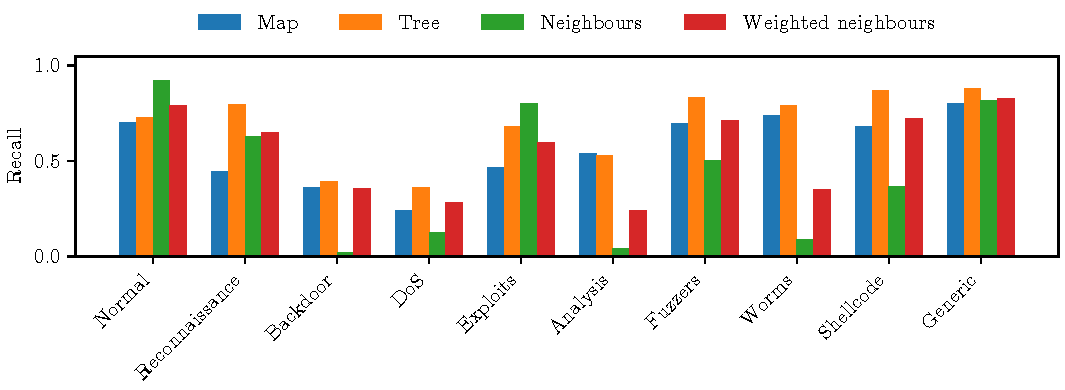
\includegraphics{figures/recall.pdf}
\caption{Per-category recall on the pooled folds}
\label{fig:recall}
\end{figure*}

The reimplemented reference classifiers reproduced the results of Assignment 2.
Assignment 2 reported a macro F-measure of 0.5760 for the tree and 0.4554 for the uniform vote, both obtained with the scikit-learn library \cite{pedregosa2011}.
The departures of 0.0012 and 0.0029 lay inside the fold standard deviations reported in both studies.

The SOM ranked differently under each measure.
Under the macro F-measure, the SOM ranked last.
Under balanced accuracy, the SOM attained 0.5680 and ranked second, ahead of both nearest-neighbour votes.
Under accuracy, the SOM ranked last with 0.6306.
The low accuracy arose because the SOM labelled 17\,123 Normal rows as Fuzzers.
Those rows formed 20.0 per cent of the Normal rows.
The disagreement between the measures followed mainly from a trade-off between recall and precision on the rare categories.

Fig.~\ref{fig:recall} shows the per-category recall of every model.
The SOM recalled Worms at 0.737, close to the 0.789 of the tree and far above the 0.088 of the uniform vote.
The SOM also recalled Shellcode at 0.683, Analysis at 0.540 and Backdoor at 0.360, in each case far above the uniform vote.
However, the precision for Worms was low.
The SOM predicted Worms for 8\,839 rows, and only 126 of those rows were Worms.
The precision for Worms was therefore 0.014, and the F-measure for Worms was 0.028.
By contrast, the tree predicted Worms for 274 rows with 135 correct predictions and attained an F-measure of 0.607 on Worms.

\begin{figure*}[tb]
\centering
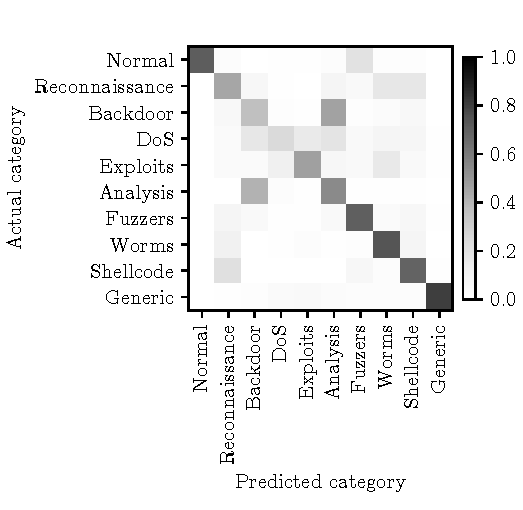
\includegraphics{figures/confusion.pdf}
\caption{Row-normalised confusion matrix of the selected map on the pooled folds}
\label{fig:cm}
\end{figure*}

The weight in \eqref{eq:weight} explained the low precision.
The ratio of the weight of Worms to the weight of Normal equalled the inverse ratio of the training counts, roughly 500.
One Worms pattern on a unit inside the neighbourhood therefore outweighed about 500 Normal patterns.
The 120 Worms training rows fell on 63 units spread across the lattice.
As a result, 212 of the 1\,024 units had a Worms count within three widths, and 17.4 per cent of the validation queries reached such a unit.
Fig.~\ref{fig:cm} confirms the effect.
The SOM labelled 17.5 per cent of the Reconnaissance rows and 16.3 per cent of the Exploits rows as Worms.
The tree avoided the effect because the tree applies the weight inside the impurity of a split.
The split instead isolates a region that contains Worms, without favouring Worms wherever a Worms row lies nearby.

Fig.~\ref{fig:cm} also shows a symmetric confusion between Backdoor and Analysis.
The SOM labelled 46.0 per cent of the Backdoor rows as Analysis and 40.8 per cent of the Analysis rows as Backdoor.
Assignment 2 reported the same pair as the main source of error of the tree, at 43.8 per cent in each direction.
The two categories therefore overlapped in the input space itself, and the confusion was not specific to the SOM.

The gap between the SOM and the uniform nearest-neighbour vote was consistent with the compression of the training data.
The nearest-neighbour vote uses the original training rows, while the SOM uses 1\,024 codebook vectors.
In the SOM, no codebook vector represents Worms, so the label of Worms remains available only through the histograms and the vote weight.
The evidence supports the compression as a likely contributor to the gap.
However, the study did not isolate the compression from the other differences between the two models.
The answer to the fourth research question is that the SOM scored below both references under the macro F-measure but detected the rare categories better than the uniform vote.

\subsection{Limit imposed by label ambiguity}
The deduplicated table contained 153\,684 distinct input vectors.
Of those vectors, 2\,445 carried more than one category.
A total of 11\,506 rows lay on such a vector, a share of 7.07 per cent.
Assignment of the majority category of each vector to every copy yielded an accuracy of 0.9443.
All reported accuracies lay at least 0.17 below the bound, so the bound did not explain the gap between the models.
The gap therefore reflected the models rather than the data.

In summary, the selection produced a $32\times32$ map with a narrow convergence width, the inverse-frequency vote and the class cap.
The map detected the rare categories with low precision, and the tree remained the best model under the macro F-measure.

\section{Conclusions}
\label{sec:conclusions}
The study trained a self-organising map (SOM) on the UNSW-NB15 network intrusion data set without the category label.
Labels were attached to the trained map, and the labelled map was compared with the nearest-neighbour classifier and the classification tree of Assignment 2.
Five findings emerged.

The first finding concerned the input representation.
The Euclidean fit of the SOM required both the logarithm and standardisation.
Together, the two transforms raised the validation macro F-measure from 0.1688 to 0.3284.

The second finding concerned the size and the training of the map.
The validation macro F-measure showed a plateau from roughly 576 units, while the quantisation error continued to decrease.
The quantisation error therefore did not identify the useful size of the map.
The convergence width was the only training setting with an effect larger than the initialisation noise.
A narrow width improved the macro F-measure but nearly tripled the topographic error.

The third finding concerned the labelling of the map.
Clustering of the codebook by the method of Ward lowered the macro F-measure at every number of clusters.
Each of the three largest categories occupied more than one region of the map, so every merge discarded category information.
The inverse-frequency vote matched the majority rule on the macro F-measure and raised the balanced accuracy from 0.3886 to 0.5679.

The fourth finding concerned the rare categories.
The vote raised the recall of Worms to 0.737 on the five folds.
However, the vote predicted Worms for 8\,839 rows, and only 126 of those rows were Worms.
The gain in recall therefore came with a very low precision.
A cap on the number of training patterns per category changed the macro F-measure by less than the initialisation noise.

The fifth finding concerned the comparison.
The SOM attained a five-fold macro F-measure of 0.4135, compared with 0.4525 for the uniform nearest-neighbour vote and 0.5772 for the tree.
The class-weighted tree remained the best model under the macro F-measure.

Three directions extend the study.
A milder vote weight, such as the square root of $\alpha_c$, would lie between the uniform and the inverse-frequency vote.
The milder weight would test whether precision on the rare categories improves.
A hierarchical SOM, as used by Kayacik \emph{et al.}, would allow a second map to separate the rare categories within the units that the first map assigns to the frequent categories.
Finally, training ten maps on bootstrap samples would show whether an ensemble reduces the sensitivity of the map to the initialisation.

\raggedbottom
\appendices
\section{Acronyms}
The acronyms used in the report are listed alphabetically below.

\noindent DoS: denial of service.\\
SOM: self-organising map.\\
UNSW-NB15: the network intrusion data set released by Moustafa and Slay.

\section{Symbols}
Table~\ref{tab:symbols} lists the symbols alphabetically, with each Greek letter sorted by name.

\begin{table}[H]
\caption{Symbols}
\label{tab:symbols}
\centering
\scriptsize
\begin{tabular}{lp{0.72\columnwidth}}
\toprule
Symbol & Meaning \\
\midrule
$A$, $B$ & Clusters of units \\
$\alpha_c$ & Inverse-frequency weight of category $c$ \\
$b(p)$ & Best-matching unit of pattern $p$ \\
$b'(p)$ & Second-best unit of pattern $p$ \\
$C$ & Number of categories \\
$c$ & Category index \\
$d_{AB}$ & Ward increase for the merge of $A$ and $B$ \\
$\delta_p$ & Indicator that $b(p)$ and $b'(p)$ are not adjacent \\
$E$ & Number of ordering epochs \\
$\eta(t)$ & Learning rate at epoch $t$ \\
$F_c$ & F-measure of category $c$ \\
$\bar{F}$ & Macro F-measure \\
$G$ & Gini index of a node, with $G_L$ and $G_R$ for the children \\
$\mathbf{g}_u$ & Lattice coordinate of unit $u$ \\
$k$ & Number of nearest neighbours \\
$m_c$ & Number of training patterns in category $c$ \\
$\boldsymbol{\mu}_A$ & Pattern-weighted mean codebook vector of cluster $A$ \\
$n_v$, $n_A$ & Number of training patterns won by unit $v$ or by cluster $A$ \\
$\omega$ & Pattern weight at a node, with $\omega_L$ and $\omega_R$ for the children \\
$P$ & Number of training patterns \\
$p$ & Pattern index \\
$\phi_{vu}(t)$ & Neighbourhood kernel between units $v$ and $u$ \\
$\pi_c$ & Precision of category $c$ \\
$Q$ & Quantisation error \\
$\rho_c$ & Recall of category $c$ \\
$\bar{\rho}$ & Balanced accuracy \\
$s$ & Standard deviation of $\bar{F}$ over the folds \\
$\sigma(t)$ & Neighbourhood width at epoch $t$ \\
$T$ & Topographic error \\
$t$ & Epoch index \\
$\tau$ & Time constant of the decays \\
$\theta_c$ & Weighted share of category $c$ at a node \\
$u$, $v$ & Unit indices, with $v$ the winning unit \\
$\mathbf{w}_u$ & Codebook vector of unit $u$ \\
$\mathbf{z}_p$ & Input vector of pattern $p$ \\
$\bar{\mathbf{z}}_v$ & Mean input vector of the patterns won by unit $v$ \\
\bottomrule
\end{tabular}
\end{table}

\begin{thebibliography}{99}
\bibitem{breiman1984}
L.~Breiman, J.~H. Friedman, R.~A. Olshen, and C.~J. Stone, \emph{Classification and Regression Trees}. Belmont, CA: Wadsworth, 1984.

\bibitem{brodersen2010}
K.~H. Brodersen, C.~S. Ong, K.~E. Stephan, and J.~M. Buhmann, ``The balanced accuracy and its posterior distribution,'' in \emph{Proceedings of the 20th International Conference on Pattern Recognition}, Istanbul, Turkey, 2010, pp.~3121--3124.

\bibitem{cover1967}
T.~M. Cover and P.~E. Hart, ``Nearest neighbor pattern classification,'' \emph{IEEE Transactions on Information Theory}, vol.~13, no.~1, pp.~21--27, 1967.

\bibitem{engelbrecht2007}
A.~P. Engelbrecht, \emph{Computational Intelligence: An Introduction}, 2nd~ed. Chichester: Wiley, 2007.

\bibitem{harris2020}
C.~R. Harris, K.~J. Millman, S.~J. van~der Walt, R.~Gommers, P.~Virtanen, D.~Cournapeau, E.~Wieser, J.~Taylor, S.~Berg, N.~J. Smith, R.~Kern, M.~Picus, S.~Hoyer, M.~H. van~Kerkwijk, M.~Brett, A.~Haldane, J.~Fern\'andez del R\'io, M.~Wiebe, P.~Peterson, P.~G\'erard-Marchant, K.~Sheppard, T.~Reddy, W.~Weckesser, H.~Abbasi, C.~Gohlke, and T.~E. Oliphant, ``Array programming with NumPy,'' \emph{Nature}, vol.~585, no.~7825, pp.~357--362, 2020.

\bibitem{hastie2009}
T.~Hastie, R.~Tibshirani, and J.~Friedman, \emph{The Elements of Statistical Learning}, 2nd~ed. New York: Springer, 2009.

\bibitem{he2009}
H.~He and E.~A. Garcia, ``Learning from imbalanced data,'' \emph{IEEE Transactions on Knowledge and Data Engineering}, vol.~21, no.~9, pp.~1263--1284, 2009.

\bibitem{kayacik2007}
H.~G. Kayacik, A.~N. Zincir-Heywood, and M.~I. Heywood, ``A hierarchical SOM-based intrusion detection system,'' \emph{Engineering Applications of Artificial Intelligence}, vol.~20, no.~4, pp.~439--451, 2007.

\bibitem{kiviluoto1996}
K.~Kiviluoto, ``Topology preservation in self-organizing maps,'' in \emph{Proceedings of the International Conference on Neural Networks}, vol.~1, Washington, DC, 1996, pp.~294--299.

\bibitem{kohavi1995}
R.~Kohavi, ``A study of cross-validation and bootstrap for accuracy estimation and model selection,'' in \emph{Proceedings of the 14th International Joint Conference on Artificial Intelligence}, vol.~2, Montreal, Canada, 1995, pp.~1137--1143.

\bibitem{kohonen1990}
T.~Kohonen, ``The self-organizing map,'' \emph{Proceedings of the IEEE}, vol.~78, no.~9, pp.~1464--1480, 1990.

\bibitem{kohonen2001}
T.~Kohonen, \emph{Self-Organizing Maps}, 3rd~ed. Berlin: Springer, 2001.

\bibitem{lam2015}
S.~K. Lam, A.~Pitrou, and S.~Seibert, ``Numba: A LLVM-based Python JIT compiler,'' in \emph{Proceedings of the Second Workshop on the LLVM Compiler Infrastructure in HPC}, Austin, TX, 2015, pp.~1--6.

\bibitem{moustafa2015}
N.~Moustafa and J.~Slay, ``UNSW-NB15: A comprehensive data set for network intrusion detection systems,'' in \emph{Proceedings of the Military Communications and Information Systems Conference}, Canberra, Australia, 2015, pp.~1--6.

\bibitem{moustafa2016}
N.~Moustafa and J.~Slay, ``The evaluation of network anomaly detection systems: Statistical analysis of the UNSW-NB15 data set and the comparison with the KDD99 data set,'' \emph{Information Security Journal: A Global Perspective}, vol.~25, no.~1--3, pp.~18--31, 2016.

\bibitem{pedregosa2011}
F.~Pedregosa, G.~Varoquaux, A.~Gramfort, V.~Michel, B.~Thirion, O.~Grisel, M.~Blondel, P.~Prettenhofer, R.~Weiss, V.~Dubourg, J.~Vanderplas, A.~Passos, D.~Cournapeau, M.~Brucher, M.~Perrot, and E.~Duchesnay, ``Scikit-learn: Machine learning in Python,'' \emph{Journal of Machine Learning Research}, vol.~12, pp.~2825--2830, 2011.

\bibitem{ramadas2003}
M.~Ramadas, S.~Ostermann, and B.~Tjaden, ``Detecting anomalous network traffic with self-organizing maps,'' in \emph{Proceedings of the International Symposium on Recent Advances in Intrusion Detection}, Pittsburgh, PA, 2003, pp.~36--54.

\bibitem{sokolova2009}
M.~Sokolova and G.~Lapalme, ``A systematic analysis of performance measures for classification tasks,'' \emph{Information Processing and Management}, vol.~45, no.~4, pp.~427--437, 2009.

\bibitem{ultsch1990}
A.~Ultsch and H.~P. Siemon, ``Kohonen's self organizing feature maps for exploratory data analysis,'' in \emph{Proceedings of the International Neural Network Conference}, Paris, France, 1990, pp.~305--308.

\bibitem{vesanto2000}
J.~Vesanto and E.~Alhoniemi, ``Clustering of the self-organizing map,'' \emph{IEEE Transactions on Neural Networks}, vol.~11, no.~3, pp.~586--600, 2000.

\bibitem{ward1963}
J.~H. Ward, ``Hierarchical grouping to optimize an objective function,'' \emph{Journal of the American Statistical Association}, vol.~58, no.~301, pp.~236--244, 1963.
\end{thebibliography}

\end{document}
